\documentclass[14pt]{extbook}
\usepackage{multicol, enumerate, enumitem, hyperref, color, soul, setspace, parskip, fancyhdr} %General Packages
\usepackage{amssymb, amsthm, amsmath, bbm, latexsym, units, mathtools} %Math Packages
\everymath{\displaystyle} %All math in Display Style
% Packages with additional options
\usepackage[headsep=0.5cm,headheight=12pt, left=1 in,right= 1 in,top= 1 in,bottom= 1 in]{geometry}
\usepackage[usenames,dvipsnames]{xcolor}
\usepackage{dashrule}  % Package to use the command below to create lines between items
\newcommand{\litem}[1]{\item#1\hspace*{-1cm}\rule{\textwidth}{0.4pt}}
\pagestyle{fancy}
\lhead{Progress Quiz 3}
\chead{}
\rhead{Version C}
\lfoot{}
\cfoot{}
\rfoot{Fall 2020}
\begin{document}

\begin{enumerate}
\litem{
Solve the equation below. Then, choose the interval that contains the solution.\[ -15(2x + 7) = -13(-8x + 5) \]\begin{enumerate}[label=\Alph*.]
\item \( x \in [-0.47, 0.66] \)
\item \( x \in [0.57, 1.53] \)
\item \( x \in [1.89, 2.45] \)
\item \( x \in [-2.45, -1.08] \)
\item \( \text{There are no real solutions.} \)

\end{enumerate} }
\litem{
First, find the equation of the line containing the two points below. Then, write the equation as $ y=mx+b $ and choose the intervals that contain $m$ and $b$.\[ (-6, 6) \text{ and } (10, -4) \]\begin{enumerate}[label=\Alph*.]
\item \( m \in [-1.62, 0.38] \hspace*{3mm} b \in [-9.25, -0.25] \)
\item \( m \in [-0.38, 7.62] \hspace*{3mm} b \in [-12.25, -4.25] \)
\item \( m \in [-1.62, 0.38] \hspace*{3mm} b \in [-15, -11] \)
\item \( m \in [-1.62, 0.38] \hspace*{3mm} b \in [2.25, 6.25] \)
\item \( m \in [-1.62, 0.38] \hspace*{3mm} b \in [12, 14] \)

\end{enumerate} }
\litem{
Solve the linear equation below. Then, choose the interval that contains the solution.\[ \frac{-3x -8}{5} - \frac{5x -7}{8} = \frac{-7x + 6}{7} \]\begin{enumerate}[label=\Alph*.]
\item \( x \in [-15.81, -13.81] \)
\item \( x \in [-34.11, -30.11] \)
\item \( x \in [-2.58, -0.58] \)
\item \( x \in [-9.03, -4.03] \)
\item \( \text{There are no real solutions.} \)

\end{enumerate} }
\litem{
Find the equation of the line described below. Write the linear equation as $ y=mx+b $ and choose the intervals that contain $m$ and $b$.\[ \text{Parallel to } 4 x + 3 y = 5 \text{ and passing through the point } (-8, 6). \]\begin{enumerate}[label=\Alph*.]
\item \( m \in [-1.47, -0.93] \hspace*{3mm} b \in [-4.67, -3.67] \)
\item \( m \in [1.01, 1.49] \hspace*{3mm} b \in [15.67, 20.67] \)
\item \( m \in [-0.83, -0.38] \hspace*{3mm} b \in [-4.67, -3.67] \)
\item \( m \in [-1.47, -0.93] \hspace*{3mm} b \in [11, 16] \)
\item \( m \in [-1.47, -0.93] \hspace*{3mm} b \in [2.67, 6.67] \)

\end{enumerate} }
\litem{
Find the equation of the line described below. Write the linear equation as $ y=mx+b $ and choose the intervals that contain $m$ and $b$.\[ \text{Parallel to } 8 x - 7 y = 5 \text{ and passing through the point } (-9, 7). \]\begin{enumerate}[label=\Alph*.]
\item \( m \in [1.12, 2] \hspace*{3mm} b \in [-17.68, -16.87] \)
\item \( m \in [1.12, 2] \hspace*{3mm} b \in [15.53, 16.09] \)
\item \( m \in [-0.63, 0.98] \hspace*{3mm} b \in [16.4, 17.85] \)
\item \( m \in [-2.14, -0.42] \hspace*{3mm} b \in [-3.68, -3.22] \)
\item \( m \in [1.12, 2] \hspace*{3mm} b \in [16.4, 17.85] \)

\end{enumerate} }
\litem{
Solve the linear equation below. Then, choose the interval that contains the solution.\[ \frac{-3x + 8}{3} - \frac{-9x -9}{4} = \frac{8x -9}{7} \]\begin{enumerate}[label=\Alph*.]
\item \( x \in [1.1, 5.1] \)
\item \( x \in [-15.89, -11.89] \)
\item \( x \in [-61.89, -54.89] \)
\item \( x \in [-245.67, -240.67] \)
\item \( \text{There are no real solutions.} \)

\end{enumerate} }
\litem{
Write the equation of the line in the graph below in Standard form $Ax+By=C$. Then, choose the intervals that contain $A, B, \text{ and } C$.
\begin{center}
    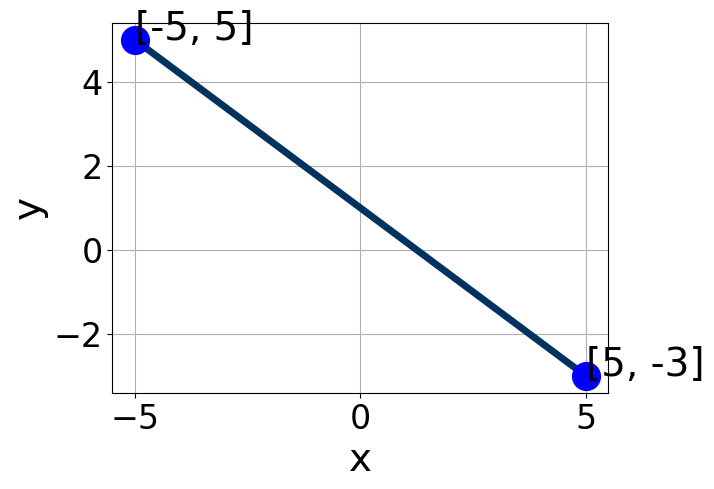
\includegraphics[width=0.5\textwidth]{../Figures/linearGraphToStandardCopyC.png}
\end{center}
\begin{enumerate}[label=\Alph*.]
\item \( A \in [-7.7, -4.4], \hspace{3mm} B \in [1.43, 3.05], \text{ and } \hspace{3mm} C \in [3.5, 7.6] \)
\item \( A \in [-2.7, -0.9], \hspace{3mm} B \in [-1.2, -0.41], \text{ and } \hspace{3mm} C \in [-5.5, -1.6] \)
\item \( A \in [4.4, 5.7], \hspace{3mm} B \in [1.43, 3.05], \text{ and } \hspace{3mm} C \in [3.5, 7.6] \)
\item \( A \in [-2.7, -0.9], \hspace{3mm} B \in [0.86, 1.44], \text{ and } \hspace{3mm} C \in [1.3, 3.7] \)
\item \( A \in [4.4, 5.7], \hspace{3mm} B \in [-2.78, -1.11], \text{ and } \hspace{3mm} C \in [-10.5, -5.7] \)

\end{enumerate} }
\litem{
First, find the equation of the line containing the two points below. Then, write the equation as $ y=mx+b $ and choose the intervals that contain $m$ and $b$.\[ (10, 6) \text{ and } (7, -11) \]\begin{enumerate}[label=\Alph*.]
\item \( m \in [1.67, 6.67] \hspace*{3mm} b \in [46.67, 51.67] \)
\item \( m \in [1.67, 6.67] \hspace*{3mm} b \in [-6, 3] \)
\item \( m \in [1.67, 6.67] \hspace*{3mm} b \in [-50.67, -48.67] \)
\item \( m \in [1.67, 6.67] \hspace*{3mm} b \in [-18, -15] \)
\item \( m \in [-15.67, -1.67] \hspace*{3mm} b \in [23.67, 33.67] \)

\end{enumerate} }
\litem{
Solve the equation below. Then, choose the interval that contains the solution.\[ -10(5x -17) = -13(-2x -18) \]\begin{enumerate}[label=\Alph*.]
\item \( x \in [-1.84, 0.16] \)
\item \( x \in [15.83, 17.83] \)
\item \( x \in [3.32, 6.32] \)
\item \( x \in [-5.32, -3.32] \)
\item \( \text{There are no real solutions.} \)

\end{enumerate} }
\litem{
Write the equation of the line in the graph below in Standard form $Ax+By=C$. Then, choose the intervals that contain $A, B, \text{ and } C$.
\begin{center}
    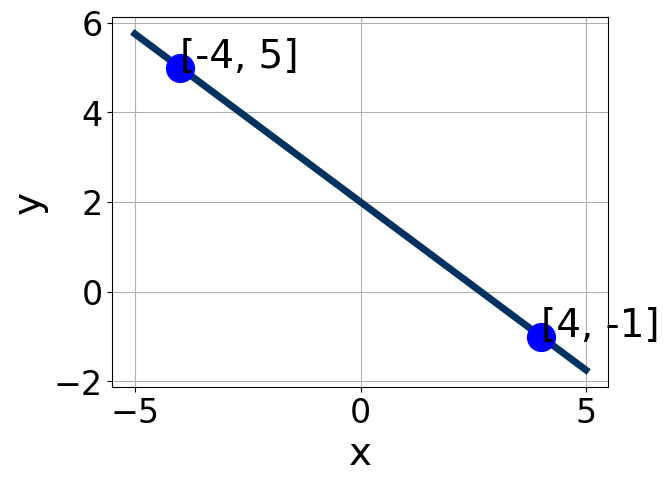
\includegraphics[width=0.5\textwidth]{../Figures/linearGraphToStandardC.png}
\end{center}
\begin{enumerate}[label=\Alph*.]
\item \( A \in [-4.25, 1.75], \hspace{3mm} B \in [-0.9, 1.1], \text{ and } \hspace{3mm} C \in [-7, -4] \)
\item \( A \in [2, 6], \hspace{3mm} B \in [-5.4, -1.2], \text{ and } \hspace{3mm} C \in [19, 22] \)
\item \( A \in [-6, -3], \hspace{3mm} B \in [3, 6.4], \text{ and } \hspace{3mm} C \in [-23, -16] \)
\item \( A \in [2, 6], \hspace{3mm} B \in [3, 6.4], \text{ and } \hspace{3mm} C \in [-23, -16] \)
\item \( A \in [-4.25, 1.75], \hspace{3mm} B \in [-1.7, -0.2], \text{ and } \hspace{3mm} C \in [0, 6] \)

\end{enumerate} }
\end{enumerate}

\end{document}